\clearpage
\setcounter{page}{1}


\appendix


\renewcommand{\thesection}{\Alph{section}}
\renewcommand{\thesubsection}{\Alph{section}.\arabic{subsection}}
\crefname{algocf}{alg.}{algs.}
\Crefname{algocf}{Algorithm}{Algorithms}
% \crefalias{section}{appendix}

\section{Code and Datasets}\label{supp:code_and_datasets}

\jvl{
The proposed KD-VDU experimentation framework is available in the Supplementary zip. This includes the DIC benchmarking that is made fully compatible with HuggingFace \textit{transformers}, even allowing arbitrary image classification models and (document) image datasets from HuggingFace \textit{hub}.\\
  The DLA benchmark is built around the \textit{Detectron2} framework, with additional scripts for efficiency evaluation, visualization, and document data preparation for downstream tasks (\Cref{algo:pseudo}).
  Downstream task experiments are made available as a fork of the original LATIN-prompt \cite{wang2023layout} implementations with additional modifications (4-bit quantization, question type ANLS evaluation, InfographicsVQA dataloader, structure-preserving OCR respecting DLA tokens).
}


\section{Implementation Details}\label{supp:implementation_details}

\subsection{DIC}

All runs are documented with hyperparameter configuration and commandline arguments in a \textit{wandb} project that will be released upon acceptance for complete transparency in experiment results and reproducibility. %\href{DistilDoc}{https://wandb.ai/jordy-vlan/DistilDoc}.

For \rvl{}, both teacher and student training is carried out for 10 epochs with a batch size of (32 ViT, 64 ResNet) and AdamW with weight decay 5e-4 and a learning rate of 1e-4 with a linear warmup of 10\%.
For \tobacco{}, the default recipe is similarly trained for 100 epochs. All experiments were performed on a single NVIDIA GeForce RTX 3090 GPU (24GB GPU vRAM).
For some feature-based KD methods, the batch size was necessarily lowered to 16 due to memory constraints.
KD method hyperparameters were cross-validated to find the best performing configuration for each method, and are listed in the main manuscript result tables.

\subsection{DLA}

In this paper, MaskRCNN detection architecture is considered with two different backbones (1) CNNs: ResNet50 and ResNet101 (2) Transformers: ViT base and ViT tiny. All the detection models are trained with Detectron2~\cite{wu2019detectron2} which uses the PyTorch deep learning library. The hyperparameters used are the following: (a) learning rate of 1e-4 (b) iterations 300k (c) optimizer: Adam (d) batch size: 16 (e) ROI heads predictions: 128 (f) NMS threshold: 0.4 (g) confidence threshold: 0.6
% In this paper, two object detection models are considered: (1) Vanilla MaskRCNN: This model is the Mask-RCNN with a ResNet(-50/101) visual backbone. (2) switching to a ViT backbone. We train instance segmentation models with the Detectron2 framework \cite{wu2019detectron2}. Models are trained for 300k iterations with a base learning rate of 1e-4 and a batch size of 512 on a single A40 GPU.
For reproducibility, we share the exact config files used for each experiment as part of the Supplementary,

\paragraph{Teacher and student model variants} \Cref{tab:vistrans,tab:resnet} indicate the differences between used teacher and student models in terms of parameterization and efficiency.

\begin{table}[h]
  \centering
  \caption{Details of Vision Transformer model variants \cite{dosovitskiy2020image}.}
  \scalebox{0.8}{
    \begin{tabular}{l|ccccc}
      \hline \multirow{2}{*}{ Variants } & \multicolumn{5}{|c}{ Settings of D/ViT }                                            \\
                                         & Layers                                   & Width & FFN  & Heads & \#Param           \\
      \hline Tiny (T)                    & 12                                       & 192   & 768  & 3     & $5.5 \mathrm{M}$  \\
      Small (S)                          & 12                                       & 384   & 1536 & 6     & $21.7 \mathrm{M}$ \\
      Base (B)                           & 12                                       & 768   & 3072 & 12    & $85.8 \mathrm{M}$ \\
      %Large (L) & 24 & 1024 & 4096 & 16 & $303.3 \mathrm{M}$ \\
      %Huge (H) & 32 & 1280 & 5120 & 16 & $632 \mathrm{M}$ \\
      \hline
    \end{tabular}}
  \label{tab:vistrans}
\end{table}

\begin{table}[h]
\centering
  \caption{Details of the efficiency of model checkpoints considered in this work.}
  \label{tab:resnet}
\begin{tabular}{llll}
\hline
\textbf{Model}                  & \textbf{GFLOPs} & \textbf{GMACs} & \textbf{Params (M)} \\ \hline
\textit{microsoft/resnet-101  }          & 15.65           & 7.8            & 42.5               \\
\textit{microsoft/resnet-50  }           & 8.21            & 4.09           & 23.51              \\
\textit{google/vit-base-patch16-224}     & 35.15           & 17.56          & 86.39              \\
\textit{microsoft/dit-base }             & 35.15           & 17.56          & 85.81              \\
\textit{WinKawaks/vit-small-patch16-224} & 9.21            & 4.6            & 21.81              \\
\textit{WinKawaks/vit-tiny-patch16-224}  & 2.51            & 1.25           & 5.56            \\ \bottomrule
\end{tabular}
\end{table}



\subsection{Downstream}

We extended the implementation of \cite{wang2023layout} to incorporate Llama-2 \cite{touvron2023llama} and build a similar dataloader for InfographicsVQA \cite{mathew2022infographicvqa}.
To enable strict compatibility, we used the same unified OCR format, DUE \cite{borchmann2021due}, for all datasets. This facilitated easy incorporation of DLA tokens into the OCR tokens without disrupting the logic behind the original layout-aware representation of document text.
As it involved zero-shot evaluation, no finetuning was attempted for this task, and while it could be left for future work, we want to iterate that we sought to explore the innate ability of LLMs to ingest DLA-enriched prompts, and not the downstream task performance itself.


\section{Task definitions}\label{sec:supp-taskdef}

To place each task in the context of document inputs, we define the following tasks and their respective inputs with common notation.
We follow notation established in \cite{van2023beyond} for document page inputs.

A \textbf{page} $p$ consists of an image $\boldsymbol{v} \in \mathbb{R}^{C \times H \times W}$ (number of channels, height, and width, respectively) with $T$ word tokens $u = \left\{w_t\right\}_{t=1}^T$ organized according to a layout structure $s = \left\{\left(x_t^1, y_t^1, x_t^2, y_t^2\right)\right\}_{t=1}^T$, typically referred to as token bounding boxes, coming from OCR or available from a born-digital document.

\subsection{DIC}\label{sec:supp-taskdef_dic}

As a prototypical instance of classification \cite{vapnik1992principles} the goal is to learn an estimator $f: \mathcal{X} \to \mathcal{Y}$ using $N$ supervised input-output pairs $(X,Y) \in \mathcal{X} \times \mathcal{Y}$ drawn \textit{iid} from an unknown joint distribution $P(X,Y)$.
In the context of DIC, the input space $\mathcal{X}$ is the set of all document images, and the output space $\mathcal{Y}$ is the set of all document classes (\eg \textit{invoice, email, form, advertisement}, \etc). The goal is to learn a function $f$ that maps a document image $x \in \mathcal{X}$ to a document class $y \in \mathcal{Y}$, such that $f(x) = y$.
\textit{Covariate shift} \cite{shimodaira2000improving} occurs when the input distribution $P(X)$ changes between the training and evaluation sets, but the conditional distribution $P(Y|X)$ remains the same. Put plainly, both sets share the same document classes, yet the visual appearance, layout and content of the document images can be different. For example, RVL-CDIP \cite{larson2022evaluating} contains more modern documents with color, whereas all \rvl{} documents are greyscale.

\subsection{DLA}\label{sec:supp-taskdef_dla}

The task of DLA can be formulated as a function that processes a document image input and outputs structured information about its logical layout elements (eg. text blocks, headers, figures, charts, plots, tables).
Let  $\mathrm{DLA}(x)$ represent the output predictions of the DLA process as a set of tuples, where each tuple $\left(b_j, c_j, p_j\right)$ represents one of $J$ detected logical layout element.
\begin{equation}
  \mathrm{DLA}(x)=\left\{\left(b_j, c_j, m_j\right)\right\}_{j=1}^J
\end{equation}
For each, $b_j$ denotes the bounding box for the $j$-th detected element, defined as $\left(x_j, y_j, w_j, h_j\right)$ (in the popular COCO format).
$c_j$ is the class label for the $j$-th element, indicating its object category. $m_j$ is a set of additional properties or information (metadata attributes, predicted scores, \textit{considered optional}) associated with the $j$-th element, which can vary depending on the type and context of the layout components.


\subsection{Zero-shot Document Visual Question Answering}\label{sec:supp-taskdef_docvqa}

Given a document $d$ and a question $q$, the goal of zero-shot DocVQA is to predict the answer $a$ to the question $q$ from the document, assuming a single document image for simplicity.
Following the text-only LLM approach in \cite{wang2023layout}, each document image requires to be translated to text, either from OCR or from a born-digital document, and the question is translated to a prompt $p$. The prompt $\boldsymbol{p}$ is a sequence of tokens that is fed to the LLM model, together with a potential task instruction, and the document image text $D$, which is structured following a heuristic procedure operating on the text tokens ($T$) and respective bounding boxes (see \Cref{supp:task_instruction}).

\section{Additional experiment results}\label{sec:supp-results}

\begin{table}[h]
  \centering
  \label{tab:results_rvl_resnet}
  \caption{Results of different KD strategies benchmarked for ResNets applied on the \rvl{} dataset. }
  \npdecimalsign{.}
  \nprounddigits{3}
  \begin{tabular}{|c|c|c|c|n{1}{3}n{1}{3}n{1}{3}|} %{|c|c|c|c||ccc|}  
    \hline Dataset        & Teacher    & Student            & Method                           & \text{ACC}                     & \text{AURC}                    & \text{ECE}                     \\  \hline %$\triangle \mathrm{Acc}$
    \rvl                  & ResNet-101 & --                 & Baseline                         & 0.819445486137153              & 0.042835121898704              & 0.016672567411534              \\
                          & --         & ResNet-50          & Baseline                         & 0.78334                        & 0.05858                        & 0.03865                        \\
\hline \hline \rvlone & ResNet-101 & \textit{ResNet-50} & Vanilla [$\tau=2.5, \alpha=0.5$] & 0.783419585489637              & 0.058696574279648              & 0.039301994115181
    \\
\hline \rvlone        & ResNet-101 &                    & NKD [$\tau=1, \gamma=1.5$]       & 0.784894622365559              & 0.062928657677387              & 0.072927374701675
    \\
\hline \rvlone        & ResNet-101 &                    & MSE                              & 0.7859196479912                & 0.058384636708256              & 0.031505212936942
    \\
\hline \rvlone        & ResNet-101 &                    & SimKD [$\varnothing$ projector]  & 0.76934423360584               & 0.067294064500561              & 0.024556334976757
    \\
\hline \rvlone        & ResNet-101 &                    & SimKD [CNN]                      & {\npboldmath}0.796669916747919 & {\npboldmath}0.052530874137723 & {\npboldmath}0.022517000562448 \\
\hline \rvlone        & ResNet-101 &                    & FitNet [middle]                  & 0.758343958598965              & 0.087305462568872              & 0.177673901604004
    \\
    \hline
  \end{tabular}
\end{table}

%placing it here for layout



\subsection{\tobacco{} results}\label{sec:supp-tobacco}

\begin{table}[h]
    \centering
    \caption{Results of different KD strategies benchmarked for ResNets applied on the \tobacco{} dataset. }
    \npdecimalsign{.}
    \nprounddigits{3}
    \begin{tabular}{|c|c|n{1}{3}n{1}{3}n{1}{3}|} %{|c|c||ccc|}  
        \hline  Student & Method          & \text{ACC}          & \text{ECE}          & \text{AURC}         \\  \hline %$\triangle \mathrm{Acc}$
        --              & Teacher         & 0.4452054794520548  & 0.1023725407268614  & 0.3595245486664192  \\
        ResNet-50       & CE              & 0.5519742143432715  & 0.0962665486513463  & 0.2559003813270729  \\
                        & CE+KD           & 0.6674053182917002  & 0.12730255396398774 & 0.14946885963574724 \\
                        & NKD             & 0.435535858178888   & 0.0760288046947609  & 0.3302691196364132  \\
                        & MSE             & 0.39927477840451253 & 0.08282232649870494 & 0.3785836239288307  \\
                        & SimKD [CLS+MLP] & 0.1764705882352941  & 0.2504398388357339  & 0.7675172798729214  \\
                        & SimKD [CNN]     & 0.314262691377921   & 0.1029121866727384  & 0.4290104103828126  \\
                        & FitNet          & 0.5769540692989524  & 0.0849604828764987  & 0.2191476496623834  \\
        \hline
    \end{tabular}
\end{table}

\begin{table}[h]
    \centering
    \caption{Results of different KD strategies benchmarked for ViT-B applied on the \tobacco{} datasets. }
    \npdecimalsign{.}
    \nprounddigits{3}
    \begin{tabular}{|c|c|n{1}{3}n{1}{3}n{1}{3}|} %{|c|c||ccc|}  
        \hline  Student & Method          & \text{ACC}         & \text{ECE}          & \text{AURC}          \\  \hline %$\triangle \mathrm{Acc}$
                        & Teacher         & 0.8759065269943593 & 0.08187206812541135 & 0.040448066777990316 \\
        ViT-S           & CE              & 0.7832393231265109 & 0.0955075391183256  & 0.0711374806067261   \\
                   & CE+KD           & 0.8140388575521533 & 0.07176496666726945 & 0.0633904758649212   \\
                   & NKD             & 0.8029814665592264 & 0.0938344161588275  & 0.0662325254143168   \\
                   & MSE             & 0.8070104754230459 & 0.1605649162609187  & 0.0618856440822465   \\
                   & SimKD [CNN]     & 0.8360193392425463 & 0.1251863664816119  & 0.0724005793664524   \\
                   & FitNet          & 0.8207091055600322 & 0.1509634972002888  & 0.0588491465898949   \\
        ViT-T            & NKD             & 0.7917002417405318 & 0.0641079216018787  & 0.069245891963159    \\
                    & MSE             & 0.798146655922643  & 0.1984227054859725  & 0.0735070428832557   \\
                    & SimKD [CLS+MLP] & 0.8106365834004835 & 0.5985289354066422  & 0.0648787085907035   \\
                    & SimKD [CNN]     & 0.8098307816277196 & 0.1354849092740382  & 0.0809560984015164   \\
                    & FitNet          & 0.8049959709911362 & 0.1597730596636112  & 0.0699693282483987   \\
        \hline
    \end{tabular}
\end{table}


\begin{table}[h]
    \centering
    \caption{Results of different KD strategies benchmarked for DiT-B applied on the \tobacco{} dataset. }
    \npdecimalsign{.}
    \nprounddigits{3}
    \begin{tabular}{|c|c|n{1}{3}n{1}{3}n{1}{3}|} %{|c|c||ccc|}  
        \hline  Student & Method          & \text{ACC}         & \text{ECE}          & \text{AURC}          \\  \hline %$\triangle \mathrm{Acc}$
                        & Teacher         & 0.9157937147461724 & 0.10934226214285338 & 0.020224875980761052 \\
        ViT-S           & CE              & 0.8203062046736502 & 0.0814063729152479  & 0.0588624099543952   \\
                        & CE+KD           & 0.8247381144238517 & 0.0862504579937333  & 0.0640506857361909   \\
                        & NKD             & 0.8134568896051572 & 0.1005910211374066  & 0.0546015365917559   \\
                        & MSE             & 0.8178887993553586 & 0.0899262672633917  & 0.0628544844656569   \\
                        & SimKD [CLS+MLP] & 0.8287671232876712 & 0.153417345835834   & 0.0564420474488556   \\
                        & SimKD [CNN]     & 0.8102336825141015 & 0.1439121554303226  & 0.0616198570583999   \\
                        & FitNet          & 0.8267526188557615 & 0.1518501442204935  & 0.0672843465750516   \\
        ViT-T           & CE              & 0.8098307816277196 & 0.0661681695247637  & 0.0654695722097237   \\
                        & CE+KD           & 0.8158742949234489 & 0.0783952415517796  & 0.0653438875243606   \\
                        & NKD             & 0.8074133763094279 & 0.0870619831212003  & 0.0627697740360264   \\
                        & MSE             & 0.8110394842868655 & 0.07172337819212    & 0.0612593916183559   \\
                        & SimKD [CLS+MLP] & 0.7784045124899275 & 0.1618730481729019  & 0.0932069554917277   \\
                        & SimKD [CNN]     & 0.7832393231265109 & 0.1871144099522751  & 0.079314938932642    \\
                        & FitNet          & 0.7929089443996776 & 0.1681748113019345  & 0.0765789086236187   \\
        \hline
    \end{tabular}
\end{table}



\subsection{\prima{} results}\label{sec:supp-prima}

\begin{table}[h]
\centering
\caption{Results for DLA-KD experiments on \prima{} dataset.}
\label{res:prima}
\begin{tabular}{@{}cccc@{}}
\toprule
\textbf{Teacher} & \textbf{Student} & \textbf{Method} & \textbf{mAP} \\ \midrule
Vit-B            & -                & Teacher        &         36.01     \\ %interpolated
Resnet-101       & -                & Teacher        & 38.34        \\
-                & ViT-T            & Baseline        &   32.64           \\ %interpolated
-                & Resnet-50        & Baseline        & 35.61        \\
                 &                  &                 &              \\
Resnet-101       & Resnet-50        & SimKD           & 35.00           \\
                 &                  & ReviewKD        & 34.31        \\
Vit-B            & ViT-T            & SimKD           &       32.05      \\ %interpolated
                 &                  & ReviewKD        &     31.94         \\ %interpolated 
                 \bottomrule
\end{tabular}
\end{table}


% Assumption:
% many DLA bboxes (start and end) spread over the whole document, better to iterate over OCR tokens and check DLA bboxes in inner loop
% \# optimization: sort DLA\_pred start and end positions; and insert them in order
% \# give naive implementation here; describe some optimizations and assumptions outside; e.g., sorting to make updates of positions and line ranges easier
% Our proposed algorithm has a time complexity of at least $O(N(M+L))$ and a space complexity of $O(NM)$



\subsection{RVL-CDIP-N results}\label{sec:supp-N}

\begin{table*}[h]
  \centering
  \caption{Evaluation including relative runtime of KD methods on \textit{RVL-CDIP-N}, where from left-to-right results are grouped per KD strategy, per backbone, per student size.}
  \label{tab:rvl_n}
  \begin{tabular}{ccc}
    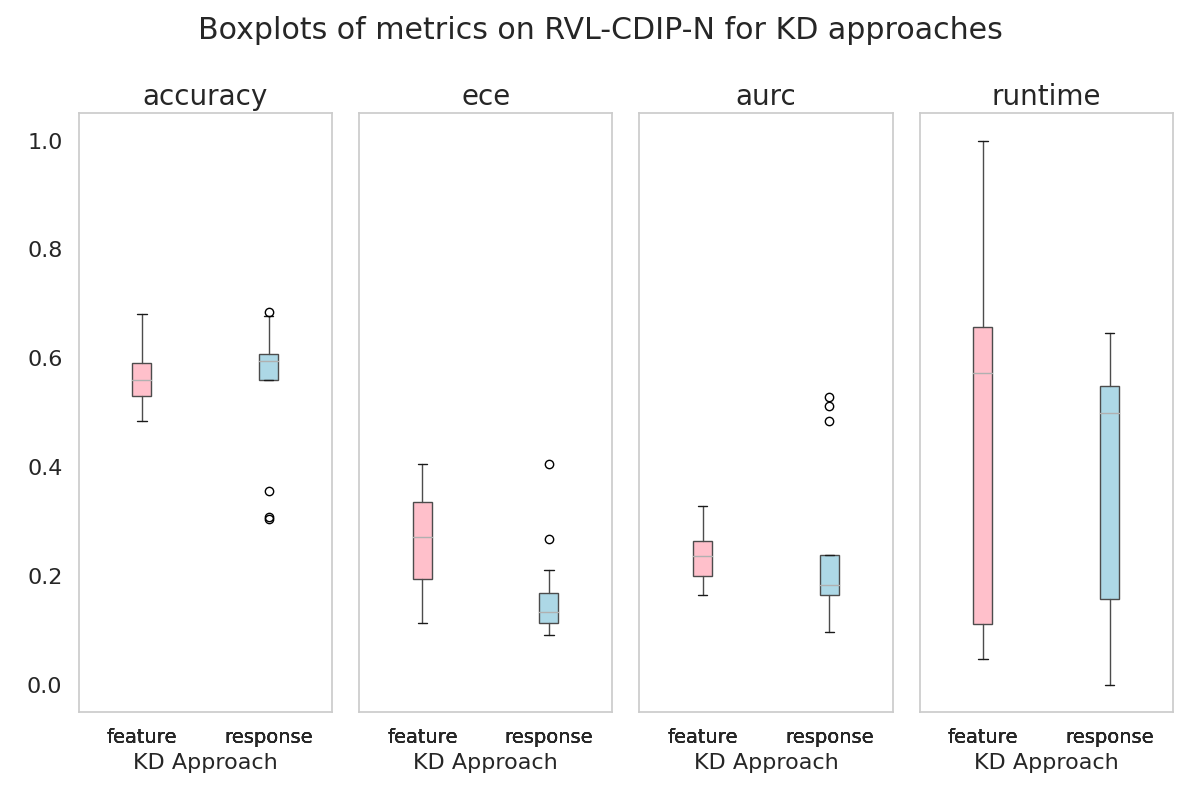
\includegraphics[width=0.33\textwidth]{images/N_results_perKDapproach.png}               &
    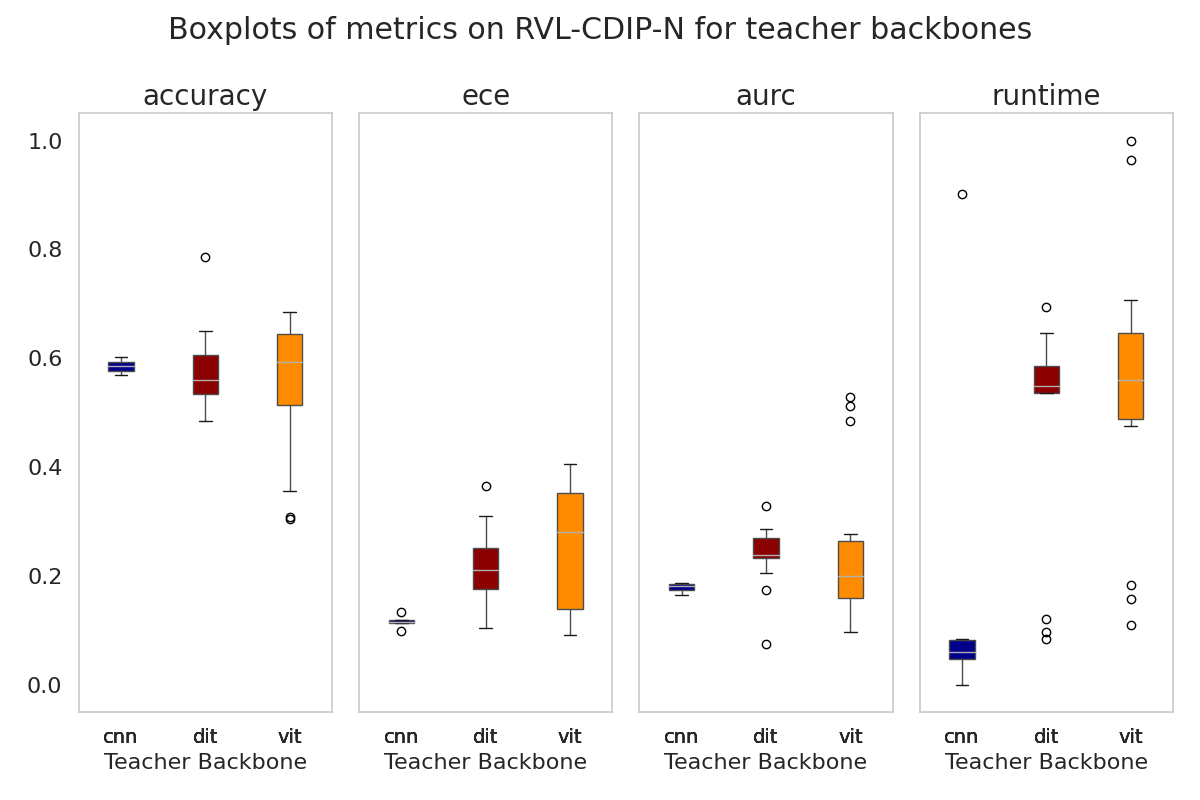
\includegraphics[width=0.33\textwidth]{images/N_results_perbackboneincludingteacher.png} &
    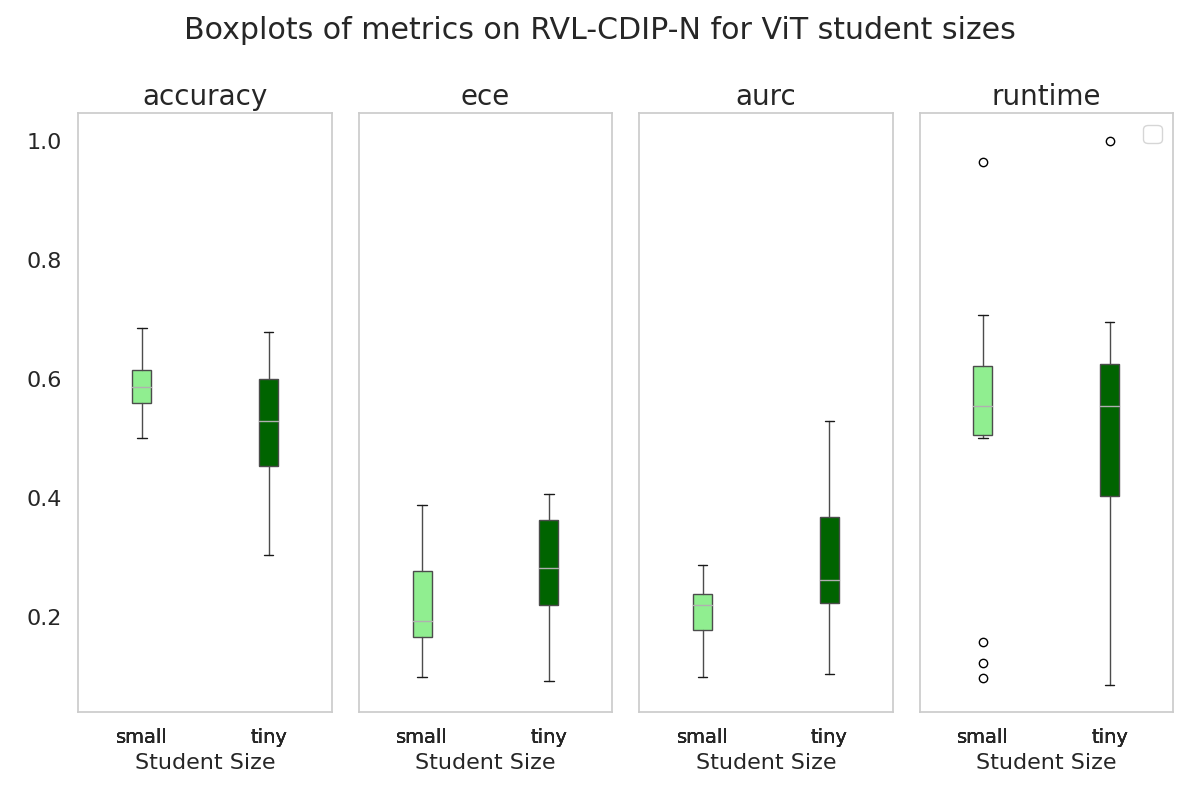
\includegraphics[width=0.33\textwidth]{images/N_results_perstudentsizes.png}               \\
  \end{tabular}
\end{table*}

%averaged
\begin{table}[h]
  \centering
\caption{Results for KD methods when averaged over architectures and student sizes on \textit{RVL-CDIP-N}.}
  \label{tab:N-averaged}
\npdecimalsign{.}
\nprounddigits{3}
\begin{tabular}{|c|n{1}{3}n{1}{3}n{1}{3}|}\toprule
KD method       & \text{ACC}          & \text{ECE}         & \text{AURC}          \\
\toprule
    Teacher         & 0.6112774451097804  & 0.11991748103719505 & 0.15233393563537376 \\
    CE              & 0.5728542914171657  & 0.11916570214335309 & 0.2153090718245799  \\ \hline
    CE+KD           & 0.519294743845642   & 0.18391029421222735 & 0.29761847107836364 \\
    NKD             & 0.5242015968063872  & {\npboldmath}0.1371122426622939  & 0.25916237807196807 \\
    MSE             & 0.49001996007984044 & 0.20466506234305107 & 0.3075089149168292  \\
    SimKD [CLS+MLP] & 0.6129740518962076  & 0.20244919407569956 & 0.21609770922954982 \\
    SimKD [CNN]     & {\npboldmath}0.6291417165668662  & 0.2734916702091337  & {\npboldmath}0.1967929796431719  \\
    FitNet          & 0.5338212463960966  & 0.28147035326753334 & 0.2455269397978257  \\
\bottomrule
  \end{tabular}
\end{table}

\subsection{Downstream DocVQA detail results}

\begin{figure}[h]
  \label{fig:ANLS_mAP_DLAplot}
  
\includegraphics[width=0.5\textwidth]{images/ANLS_DLAplot.png}
\end{figure}

\begin{table*}[h]
  \centering
  \label{tab:detail_dla_downstream_docvqa}
  \caption{Validation \ANLS{} (scaled to \%) of \textsc{Llama-2-7b-chat} \cite{touvron2023llama} on SP-DocVQA \cite{mathew2021docvqa}, with a KD-DLA model enriching the prompt.}
  \resizebox{\columnwidth}{!}{
    \begin{tabular}{@{}ll|c@{\extracolsep{0.25em}}>{\small}c@{\extracolsep{0.25em}}>{\small}c@{\extracolsep{0.25em}}>{\small}c@{\extracolsep{0.25em}}>{\small}c@{\extracolsep{0.25em}}>{\small}c@{\extracolsep{0.25em}}>{\small}c@{\extracolsep{0.25em}}>{\small}c@{\extracolsep{0.25em}}>{\small}c@{\extracolsep{0.25em}}>{\small}c@{}}
      \toprule
      prompt      & DLA                & ANLS  & Image/Photo & Yes/No & Figure/diagram & Form  & Free\_text & Handwritten & Layout & Others & Table/list \\ \midrule
      plain       &                    & 4.3   & 4.25        & 5.36   & 1.46           & 2.69  & 8.99       & 1.74        & 6.1    & 7.72   & 1.87       \\
      space       &                    & 4.61  & 2.97        & 0.0    & 1.25           & 3.31  & 7.55       & 2.14        & 6.48   & 8.45   & 2.59       \\
      task        &                    & 57.63 & 45.38       & 51.52  & 34.97          & 67.88 & 69.71      & 53.19       & 55.51  & 55.78  & 53.81      \\
      +DLA        & Resnet-101         & 57.76 & 43.31       & 47.02  & 35.01          & 66.84 & 70.03      & 52.27       & 57.16  & 58.77  & 52.22      \\
                  & Resnet-101         & 57.55 & 44.44       & 49.4   & 34.0           & 66.99 & 68.64      & 51.97       & 56.52  & 58.23  & 52.64      \\

                  & Resnet-50 ReviewKD & 57.76 & 43.31       & 47.02  & 35.01          & 66.84 & 70.03      & 52.27       & 57.16  & 58.77  & 52.22      \\
                  & Resnet-50 SimKD    & 57.53 & 45.45       & 51.52  & 35.28          & 67.39 & 68.73      & 52.23       & 56.71  & 56.5   & 52.2       \\

                  & Vit-B              & 58.39 & 44.43       & 41.67  & 34.81          & 66.38 & 67.82      & 52.1        & 59.19  & 55.91  & 52.79      \\
                  & Vit-T              & 58.65 & 44.7        & 50.3   & 36.19          & 67.65 & 68.0       & 52.49       & 59.29  & 57.03  & 52.72      \\

                  & Vit-T ReviewKD     & 57.96 & 45.9        & 47.32  & 33.49          & 66.68 & 68.92      & 51.15       & 58.46  & 56.32  & 51.89      \\
                  & Vit-T SimKD        & 58.58 & 45.09       & 49.43  & 34.92          & 67.28 & 70.64      & 52.19       & 58.44  & 57.68  & 52.82      \\
      task\_space &                    & 62.46 & 42.95       & 49.43  & 40.93          & 71.15 & 70.59      & 55.87       & 61.87  & 61.05  & 58.31      \\
      +DLA
                  & Resnet-101         & 61.86 & 41.51       & 48.24  & 40.63          & 71.12 & 69.39      & 54.56       & 61.38  & 58.62  & 57.48      \\
                  & Resnet-50          & 62.08 & 39.62       & 49.13  & 42.4           & 71.27 & 70.37      & 54.43       & 61.54  & 59.86  & 57.59      \\

                  & Resnet-50 ReviewKD & 62.14 & 44.09       & 42.26  & 40.39          & 70.6  & 69.69      & 53.07       & 61.8   & 60.14  & 58.29      \\
                  & Resnet-50 SimKD    & 61.95 & 43.93       & 44.97  & 40.57          & 71.02 & 70.12      & 54.95       & 61.43  & 60.74  & 57.69      \\

                  & Vit-B              & 61.2  & 44.58       & 49.13  & 40.28          & 68.95 & 68.39      & 52.81       & 61.38  & 56.44  & 56.7       \\
              & Vit-T & 58.65 & 44.7 & 50.3 & 36.19 & 67.65 & 68.0 & 52.49 & 59.29 & 57.03 & 52.72  \\ 

                  & Vit-T ReviewKD     & 61.58 & 46.25       & 46.75  & 37.84          & 69.37 & 69.27      & 53.86       & 61.5   & 58.44  & 57.63      \\
                  & Vit-T SimKD        & 61.46 & 44.79       & 48.24  & 40.25          & 69.55 & 69.95      & 53.15       & 61.0   & 58.18  & 57.05      \\
      \bottomrule
    \end{tabular}} %missing = ViT-T
\end{table*}

\begin{table*}[h]
  \centering
  \label{tab:detail_dla_downstream_infographicsvqa}
  \caption{Validation \ANLS{} (scaled to \%) of \textsc{Llama-2-7b-chat} \cite{touvron2023llama} on InfographicsVQA \cite{mathew2022infographicvqa}, with a KD-DLA model enriching the prompt.}

  \resizebox{\columnwidth}{!}{

    \begin{tabular}{@{}ll|c@{\extracolsep{0.25em}}>{\footnotesize}c@{\extracolsep{0.25em}}>{\footnotesize}c@{\extracolsep{0.25em}}>{\footnotesize}c@{\extracolsep{0.25em}}>{\footnotesize}c@{\extracolsep{0.25em}}>{\footnotesize}c@{\extracolsep{0.25em}}>{\footnotesize}c@{\extracolsep{0.25em}}>{\footnotesize}c@{\extracolsep{0.25em}}>{\footnotesize}c@{\extracolsep{0.25em}}>{\footnotesize}c@{\extracolsep{0.25em}}>{\footnotesize}c@{\extracolsep{0.25em}}>{\footnotesize}c@{\extracolsep{0.25em}}>{\footnotesize}c@{}}
      \toprule
      prompt     & DLA            & ANLS  & Arithmetic & Comparison & Counting & Figure & Map   & Multi-span & Non-extractive & Question span & Single span & Table/list & Text  & Visual/layout \\ \midrule
      plain      &                & 0.81  & 0.0        & 0.0        & 0.23     & 0.42   & 0.0   & 0.93       & 0.12           & 0.64          & 0.98        & 1.0        & 1.93  & 0.47          \\
      space      &                & 0.69  & 0.0        & 0.0        & 0.0      & 0.32   & 0.0   & 0.9        & 0.0            & 0.53          & 0.86        & 1.08       & 1.55  & 0.0           \\
      task       &                & 29.08 & 14.15      & 26.94      & 11.35    & 27.52  & 19.1  & 19.79      & 12.79          & 48.44         & 33.79       & 26.17      & 35.24 & 26.39         \\
      +DLA       & Resnet-50      & 27.94 & 14.1       & 26.21      & 10.28    & 26.19  & 20.25 & 17.7       & 12.28          & 45.14         & 32.7        & 24.79      & 34.3  & 26.96         \\
                 & Resnet-101     & 27.86 & 12.12      & 24.96      & 11.35    & 26.32  & 18.82 & 18.32      & 11.93          & 44.81         & 32.62       & 24.51      & 33.89 & 25.94         \\

  & Resnet-50 ReviewKD & 28.16 & 13.33 & 25.81 & 12.05 & 26.39 & 22.11 & 21.06 & 12.93 & 46.95 & 32.42 & 25.02 & 34.18 & 26.86  \\ 
  & Resnet-50 SimKD & 27.65 & 13.79 & 25.78 & 9.95 & 26.16 & 19.53 & 18.78 & 11.97 & 45.95 & 32.17 & 24.31 & 33.8 & 26.31  \\ 

                 & Vit-B          & 28.36 & 14.93      & 29.15      & 7.64     & 27.05  & 19.0  & 19.41      & 11.21          & 46.87         & 33.35       & 25.56      & 34.59 & 26.69         \\
                 & Vit-T          & 28.32 & 15.06      & 28.02      & 9.58     & 27.25  & 19.01 & 17.0       & 11.82          & 45.67         & 33.48       & 25.02      & 34.81 & 28.33         \\
                 & Vit-T ReviewKD & 28.23 & 13.35      & 27.7       & 10.78    & 26.39  & 20.03 & 20.4       & 11.92          & 45.95         & 32.95       & 25.9       & 35.28 & 27.46         \\
                 & Vit-T SimKD    & 28.18 & 14.82      & 26.31      & 9.6      & 26.19  & 18.96 & 18.09      & 12.51          & 45.36         & 32.87       & 24.93      & 34.71 & 30.98         \\
      task+space &                & 27.97 & 9.78       & 25.13      & 6.99     & 25.93  & 21.04 & 22.33      & 8.2            & 43.36         & 33.53       & 25.76      & 35.06 & 27.47         \\
      +DLA       & Resnet-50      & 27.14 & 8.12       & 23.78      & 6.27     & 24.68  & 18.67 & 19.26      & 7.0            & 41.95         & 33.03       & 25.93      & 34.07 & 28.48         \\
                 & Resnet-101     & 28.08 & 9.49       & 24.31      & 8.04     & 25.88  & 19.72 & 21.01      & 8.63           & 41.23         & 33.77       & 25.87      & 35.24 & 28.44         \\
  & Resnet-50 ReviewKD & 28.07 & 9.59 & 24.18 & 8.41 & 25.88 & 18.67 & 21.37 & 9.01 & 42.86 & 33.53 & 26.2 & 35.49 & 27.8  \\ 
  & Resnet-50 SimKD & 27.68 & 9.98 & 24.45 & 7.11 & 25.71 & 20.65 & 20.87 & 8.4 & 43.36 & 33.19 & 25.51 & 34.56 & 27.81  \\ 
                 
                 & Vit-B          & 28.05 & 9.92       & 25.28      & 7.83     & 26.28  & 19.0  & 21.85      & 8.82           & 41.84         & 33.54       & 25.57      & 34.6  & 29.17         \\
                 & Vit-T          & 27.0  & 9.06       & 23.19      & 7.34     & 25.81  & 21.9  & 18.9       & 8.04           & 39.82         & 32.65       & 23.69      & 33.93 & 28.33         \\
                 & Vit-T ReviewKD & 28.47 & 10.89      & 25.9       & 5.42     & 26.8   & 22.23 & 20.59      & 8.28           & 45.67         & 34.24       & 26.44      & 35.81 & 29.14         \\
                 & Vit-T SimKD    & 27.97 & 10.56      & 25.54      & 8.35     & 26.23  & 20.65 & 20.34      & 9.19           & 44.08         & 33.43       & 25.04      & 33.89 & 30.49         \\
      \bottomrule
    \end{tabular}}
\end{table*}


\subsection{Ablation experiments}

The experiments with random student weight initialization (\Cref{tab:ablation-cnn-rand,tab:ablation-vit-rand}) show that ViTs suffer more from student weight initialization, which is evidenced by an average accuracy of 0.5962 for ViT-S/T$_{\operatorname{rand}}$ compared to 0.7675 for R50$_{\operatorname{rand}}$.
When the student initialization is not dependent on pre-training, NKD pops up as a performant method, showing the versatility of response-based methods when transfer of feature representations is harder.

\begin{table*}[h]
  \centering
  \caption{Results of different KD strategies benchmarked for ViT-B teacher with \textbf{randomly} initialized ($\operatorname{rand}$) ViT students applied on the \rvl{} dataset. }
  \label{tab:ablation-vit-rand}
  \npdecimalsign{.}
  \nprounddigits{3}
  \begin{tabular}{|c|c|c|n{1}{3}n{1}{3}n{1}{3}|} %{|c|c|c|c||ccc|}  
    \hline
    Teacher     & Student                       & Method                           & \text{ACC}                      & \text{AURC}                    & \text{ECE}                     \\
    \hline %$\triangle \mathrm{Acc}$
    ViT-B\_rand & --                            & Baseline                         & 0.5402                          & 0.2354                         & 0.07762                        \\
    --          & ViT-$S_{\operatorname{rand}}$ & Vanilla [$\tau=2.5, \alpha=0.5$] & 0.612540313507838               & 0.175294857762794              & 0.220313611855066              \\
    ViT-B       &                               & NKD [$\tau=1, \gamma=1.5$]       & 0.579339483487087               & 0.193249005225908              & {\npboldmath}0.046056065677199 \\
    ViT-B       &                               & MSE                              & 0.625640641016025               & 0.158831615349294              & 0.202600974177652              \\
    ViT-B       &                               & SimKD [CLS+MLP]                  & 0.609090227255681               & 0.181137176233035              & 0.119806758243756              \\
    ViT-B       &                               & SimKD [CNN]                      & {\npboldmath} 0.681217030425761 & 0.181379503732163              & 0.297443627062409              \\
    ViT-B       &                               & FitNet [middle]                  & 0.627665691642291               & {\npboldmath}0.160859389524292 & 0.155333967824325              \\
    ViT-B       & ViT-$T_{\operatorname{rand}}$ & Vanilla [$\tau=2.5, \alpha=$]    & 0.559763994099852               & 0.211508769478741              & 0.141416511926601              \\
    ViT-B       &                               & NKD [$\tau=1, \gamma=1.5$]       & 0.55166379159479                & 0.21515473788689               & {\npboldmath}0.02545063954946  \\
    ViT-B       &                               & MSE                              & 0.5790394759869                 & {\npboldmath}0.198447223890963 & 0.232325413407598              \\
    ViT-B       &                               & SimKD [CLS+MLP]                  & 0.582014550363759               & 0.198973047339166              & 0.195824995889148              \\
    ViT-B       &                               & SimKD [CNN]                      & {\npboldmath}0.662866571664292  & 0.205125367580942              & 0.315795977829891              \\
    ViT-B       &                               & FitNet [middle]                  & 0.569964249106228               & 0.207300502853132              & 0.142680424442589              \\
    \hline
  \end{tabular}
\end{table*}


\begin{table*}[h]
  \centering
  \caption{Results of different KD strategies benchmarked for ResNet-101 teacher with \textbf{randomly} initialized ($\operatorname{rand}$) ResNet-50 students applied on the \rvl{} dataset.}
  \label{tab:ablation-cnn-rand}
  \npdecimalsign{.}
  \nprounddigits{3}
  \begin{tabular}{|c|c|c|n{1}{3}n{1}{3}n{1}{3}|} %{|c|c|c|c||ccc|}  
    \hline
    Teacher    & Student                              & Method                           & \text{ACC}                      & \text{AURC}                     & \text{ECE}                      \\
    \hline %$\triangle \mathrm{Acc}$
    R101\_rand & --                                   & Baseline                                                                                                                               \\
    --         & R50                                  & Baseline                         & 0.768619215480387               & 0.0154005468667318              & 0.0658814569730499              \\
    \hline
    \hline
    R101       & \textbf{R50$_{\operatorname{rand}}$} & Vanilla [$\tau=2.5, \alpha=0.5$] & 0.76014400360009                & {\npboldmath}0.0174754722636533 & 0.0712623406805409              \\
    R101       &                                      & NKD [$\tau=1, \gamma=1.5$]       & 0.7695942398559964              & 0.0510388437926124              & 0.0722681462728383              \\
    R101       &                                      & MSE                              & 0.76494412360309                & 0.0217444527724846              & 0.0676653037230823              \\
    R101       &                                      & SimKD [CLS+MLP]                  & 0.7659941498537464              & 0.0366757247091165              & 0.0678784568625449              \\
    R101       &                                      & SimKD [$\varnothing$ projector]  & {\npboldmath}0.7736693417335433 & 0.0247123270530981              & {\npboldmath}0.0633802504193506 \\
    R101       &                                      & FitNet [middle]                  & 0.760344008600215               & 0.1770233412769938              & 0.0777638551983715              \\
    \hline
  \end{tabular}
\end{table*}



